\documentclass[12pt,letterpaper]{article}\usepackage[]{graphicx}\usepackage[]{color}
%% maxwidth is the original width if it is less than linewidth
%% otherwise use linewidth (to make sure the graphics do not exceed the margin)
\makeatletter
\def\maxwidth{ %
  \ifdim\Gin@nat@width>\linewidth
    \linewidth
  \else
    \Gin@nat@width
  \fi
}
\makeatother

\definecolor{fgcolor}{rgb}{0.345, 0.345, 0.345}
\newcommand{\hlnum}[1]{\textcolor[rgb]{0.686,0.059,0.569}{#1}}%
\newcommand{\hlstr}[1]{\textcolor[rgb]{0.192,0.494,0.8}{#1}}%
\newcommand{\hlcom}[1]{\textcolor[rgb]{0.678,0.584,0.686}{\textit{#1}}}%
\newcommand{\hlopt}[1]{\textcolor[rgb]{0,0,0}{#1}}%
\newcommand{\hlstd}[1]{\textcolor[rgb]{0.345,0.345,0.345}{#1}}%
\newcommand{\hlkwa}[1]{\textcolor[rgb]{0.161,0.373,0.58}{\textbf{#1}}}%
\newcommand{\hlkwb}[1]{\textcolor[rgb]{0.69,0.353,0.396}{#1}}%
\newcommand{\hlkwc}[1]{\textcolor[rgb]{0.333,0.667,0.333}{#1}}%
\newcommand{\hlkwd}[1]{\textcolor[rgb]{0.737,0.353,0.396}{\textbf{#1}}}%

\usepackage{framed}
\makeatletter
\newenvironment{kframe}{%
 \def\at@end@of@kframe{}%
 \ifinner\ifhmode%
  \def\at@end@of@kframe{\end{minipage}}%
  \begin{minipage}{\columnwidth}%
 \fi\fi%
 \def\FrameCommand##1{\hskip\@totalleftmargin \hskip-\fboxsep
 \colorbox{shadecolor}{##1}\hskip-\fboxsep
     % There is no \\@totalrightmargin, so:
     \hskip-\linewidth \hskip-\@totalleftmargin \hskip\columnwidth}%
 \MakeFramed {\advance\hsize-\width
   \@totalleftmargin\z@ \linewidth\hsize
   \@setminipage}}%
 {\par\unskip\endMakeFramed%
 \at@end@of@kframe}
\makeatother

\definecolor{shadecolor}{rgb}{.97, .97, .97}
\definecolor{messagecolor}{rgb}{0, 0, 0}
\definecolor{warningcolor}{rgb}{1, 0, 1}
\definecolor{errorcolor}{rgb}{1, 0, 0}
\newenvironment{knitrout}{}{} % an empty environment to be redefined in TeX

\usepackage{alltt}
\usepackage[utf8]{inputenc}
\usepackage[margin=.7in]{geometry}
\usepackage{graphicx}
\usepackage{titling}
\usepackage{amsmath}
\usepackage{amsfonts}
\usepackage{amssymb}
\renewcommand{\theenumiv}{\arabic{enumiv}}
\setlength{\droptitle}{-5em}
\author{Maurice Diesendruck\vspace{-2ex}}
\title{StatMod2 - Hierarchical Models and Shrinkage - Genes\vspace{-1ex}}
\IfFileExists{upquote.sty}{\usepackage{upquote}}{}
\begin{document}
\maketitle

\section{Model}
First, take average of technical replicates to generate one time series for each
gene. Consider the following model for gene $j=1,\cdots,14$, in group $i=1,2,3$.

\begin{align*}
y_{ij}(t) &= \beta_{0j}+\beta_{1j}t + \epsilon_{ij}(t) \text{, where } 
  \epsilon_{ij} \sim\ N(\pmb{0}, \sigma^2\pmb{I})\\
\end{align*}

This implies the following structure:

\begin{align*}
y_j(t) &\sim\ N(X\pmb{\beta_j}, \sigma^2 I) &&\text{ where } 
  \beta_j=(\beta_{0j}, \beta_{1j})'\\
\pmb{\beta_j} &\sim\ N(\pmb{\mu_{i}}, \tau_{i}^2I) 
  &&\text{ Gene-level priors}\\
\pmb{\mu_{i}} &\sim\ N(\pmb{m_{i}}, v_{i}I)
  &&\text{ Group-level priors}\\
\tau_{i}^2 &\sim\ InvGamma(a_{i}, b_{i})
  &&\text{ Group-level priors}\\
\end{align*}

The joint posterior is as follows, and can be written group-wise. Here is it
written for group $1$.

\begin{align*}
P(\pmb{\beta_1},\pmb{\mu_1},\tau_{1}^2|\pmb{y_1}) &\propto\ 
  P(\pmb{y_1}|\pmb{\beta_1})P(\pmb{\beta_1}|\pmb{\mu_1},\tau_{1}^2)P(\pmb{\mu_1})
  P(\tau_{1}^2)\\
&\propto\ N(\pmb{y_1}|X\pmb{\beta_1}, \sigma^2 I)
  N(\pmb{\beta_1}|\pmb{\mu_1},\tau_1^2) N(\pmb{\mu_1}|\pmb{m_1},v_{i}I)
  InvGamma(\tau_{1}^2|a_1,b_1)\\
\vspace{3mm}\\
P(\pmb{\beta_1}|\cdots) &\sim\ N \Bigg( 
  \Big(\frac{X'X}{\sigma^2}+\frac{I}{\tau_1^2} \Big)^{-1}
  \Big(\frac{X'\pmb{y_1}}{\sigma^2}+\frac{I}{\tau_1^2} \Big),
  \Big(\frac{X'X}{\sigma^2}+\frac{I}{\tau_1^2} \Big)^{-1} 
  \Bigg)\\
P(\pmb{\mu_1}|\cdots) &\sim\ N \Bigg(
  \Big(\frac{I}{v_1}+\frac{I}{\tau_1^2} \Big)^{-1}
  \Big(\frac{I}{v_1}\pmb{m_1}+\frac{I}{\tau_1^2}\pmb{\beta_1} \Big),
  \Big(\frac{I}{v_1}+\frac{I}{\tau_1^2} \Big)^{-1} 
  \Bigg)\\
P(\frac{1}{\tau_1^2}) &\sim\ Ga(a_1 + 1, 
  \frac{(\pmb{\beta_1}-\pmb{\mu_1})'(\pmb{\beta_1}-\pmb{\mu_1})}{2} + b1)\\
\end{align*}


\newpage
\section{Results}
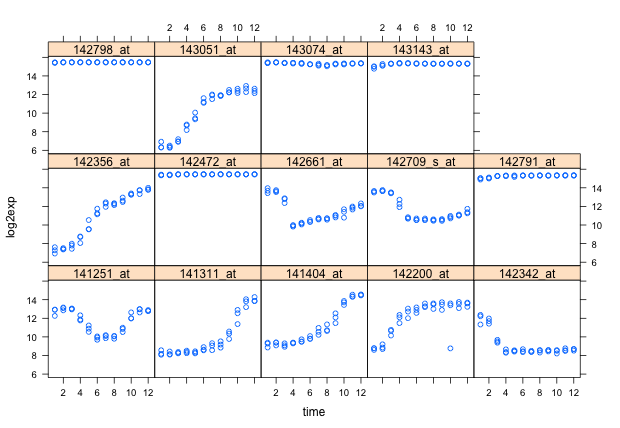
\includegraphics[height=10cm, keepaspectratio]
  {genes-groupshrink-xyplot-gene.png}\\
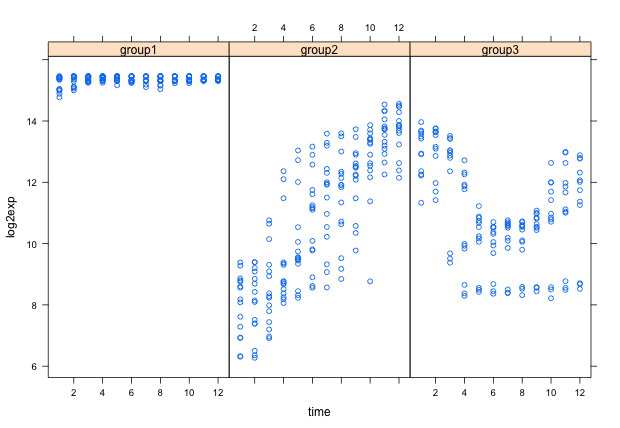
\includegraphics[height=10cm, keepaspectratio]
  {genes-groupshrink-xyplot-group.png}\\
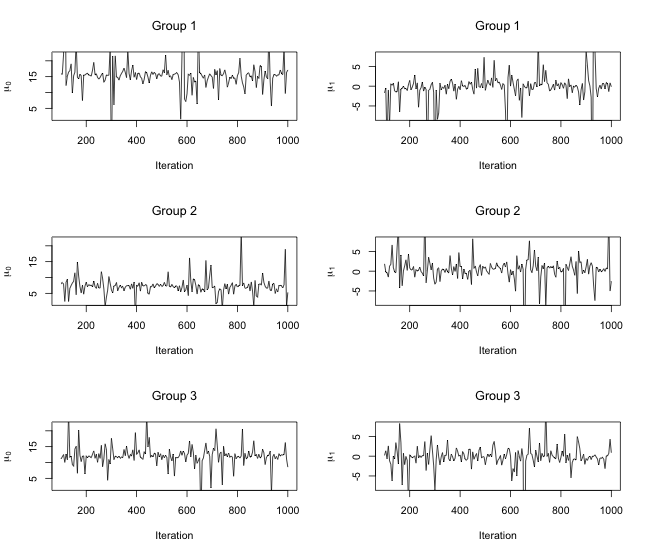
\includegraphics[width=14cm, height=20cm, keepaspectratio]
  {genes-groupshrink-mus.png}\\
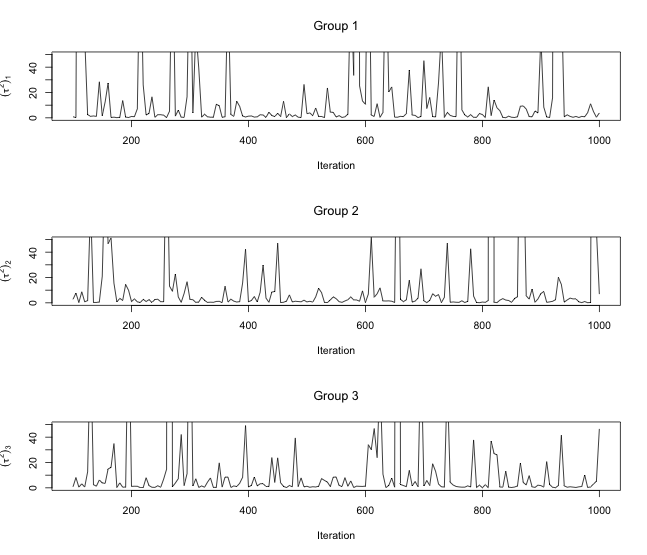
\includegraphics[width=14cm, height=20cm,keepaspectratio]
  {genes-groupshrink-taus.png}\\
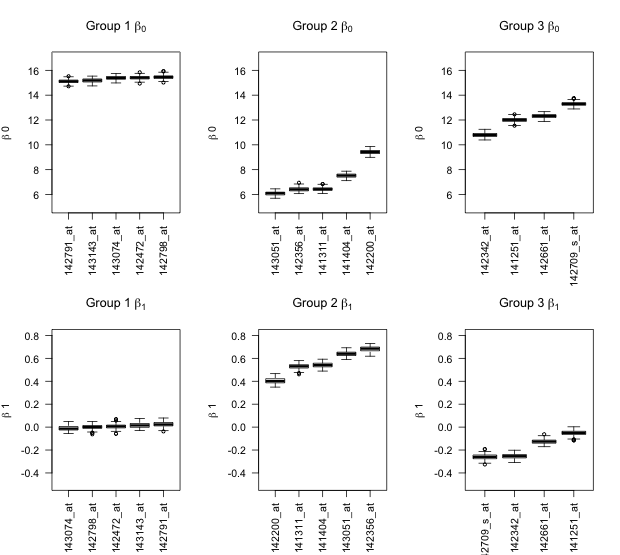
\includegraphics[width=\textwidth]
  {genes-groupshrink-betas.png}\\

\newpage
\section{Full R Code}
\begin{knitrout}
\definecolor{shadecolor}{rgb}{0.969, 0.969, 0.969}\color{fgcolor}\begin{kframe}
\begin{alltt}
\hlcom{# StatMod2 - Hierarchical Models and Shrinkage - Genes}

\hlkwd{library}\hlstd{(lattice)}
\hlkwd{library}\hlstd{(MASS)}

\hlcom{# Get data.}
\hlstd{path} \hlkwb{<-} \hlkwd{paste}\hlstd{(}\hlstr{"~/Google Drive/2. SPRING 2015/STAT MOD 2 - Prof Scott/"}\hlstd{,}
              \hlstr{"hierarch-shrinkage/genes"}\hlstd{,} \hlkwc{sep}\hlstd{=}\hlstr{""}\hlstd{)}
\hlkwd{setwd}\hlstd{(path)}
\hlstd{data} \hlkwb{<-} \hlkwd{read.csv}\hlstd{(}\hlstr{"droslong.csv"}\hlstd{)}
\hlstd{data} \hlkwb{<-} \hlstd{data[}\hlkwd{order}\hlstd{(data[,}\hlnum{1}\hlstd{], data[,}\hlnum{2}\hlstd{]),]}
\hlkwd{head}\hlstd{(data,} \hlnum{100}\hlstd{)}

\hlcom{# Quickly plot.}
\hlkwd{xyplot}\hlstd{(log2exp}\hlopt{~}\hlstd{time} \hlopt{|} \hlstd{gene,} \hlkwc{data}\hlstd{=data)}
\hlkwd{xyplot}\hlstd{(log2exp}\hlopt{~}\hlstd{time} \hlopt{|} \hlstd{group,} \hlkwc{data}\hlstd{=data)}

\hlcom{#########################################}
\hlcom{# PRELIMINARY DATA MANIPULATION}

\hlcom{# Average technical replicants, and run frequentist linear model fit for each,}
\hlcom{# to get estimates for prior on group mean and group variance.}
\hlstd{DATA.AVG.TR} \hlkwb{<-} \hlkwa{NULL}
\hlstd{lm.coefs} \hlkwb{<-} \hlkwa{NULL}
\hlstd{gene.names} \hlkwb{<-} \hlkwd{as.vector}\hlstd{(}\hlkwd{unique}\hlstd{(data}\hlopt{$}\hlstd{gene))}
\hlstd{num.names} \hlkwb{<-} \hlkwd{length}\hlstd{(gene.names)}
\hlkwa{for} \hlstd{(i} \hlkwa{in} \hlnum{1}\hlopt{:}\hlstd{num.names) \{}
  \hlcom{# Subset of data for each gene.}
  \hlstd{name} \hlkwb{<-} \hlstd{gene.names[i]}
  \hlstd{d} \hlkwb{<-} \hlstd{data[}\hlkwd{which}\hlstd{(data}\hlopt{$}\hlstd{gene}\hlopt{==}\hlstd{name),]}
  \hlstd{gene.time.avgs} \hlkwb{<-} \hlkwd{aggregate}\hlstd{(d}\hlopt{$}\hlstd{log2exp}\hlopt{~}\hlstd{d}\hlopt{$}\hlstd{time, d, mean)}
  \hlstd{d} \hlkwb{<-} \hlkwd{cbind}\hlstd{(d}\hlopt{$}\hlstd{gene[}\hlnum{1}\hlstd{], d}\hlopt{$}\hlstd{group[}\hlnum{1}\hlstd{], gene.time.avgs)}
  \hlkwd{names}\hlstd{(d)} \hlkwb{<-} \hlkwd{c}\hlstd{(}\hlstr{"gene"}\hlstd{,} \hlstr{"group"}\hlstd{,} \hlstr{"time"}\hlstd{,} \hlstr{"log2exp"}\hlstd{)}
  \hlstd{DATA.AVG.TR} \hlkwb{<-} \hlkwd{rbind}\hlstd{(DATA.AVG.TR, d)}

  \hlcom{# Also do a Frequentist exploration and store lm coefs.}
  \hlstd{fit.coefs} \hlkwb{<-} \hlkwd{lm}\hlstd{(d}\hlopt{$}\hlstd{log2exp}\hlopt{~}\hlstd{d}\hlopt{$}\hlstd{time)}\hlopt{$}\hlstd{coefficients}
  \hlstd{lm.coefs} \hlkwb{<-} \hlkwd{rbind}\hlstd{(lm.coefs,} \hlkwd{c}\hlstd{(}\hlkwd{toString}\hlstd{(name), fit.coefs,}
                                \hlkwd{toString}\hlstd{(d}\hlopt{$}\hlstd{group[}\hlnum{1}\hlstd{])))}
\hlstd{\}}
\hlcom{# Got linear model coefficients for each gene. Now average them for the prior}
\hlcom{# on group mean and group variance.}
\hlstd{just.coefs} \hlkwb{<-} \hlkwd{cbind}\hlstd{(}\hlkwd{as.numeric}\hlstd{(lm.coefs[,}\hlnum{2}\hlstd{]),} \hlkwd{as.numeric}\hlstd{(lm.coefs[,}\hlnum{3}\hlstd{]))}
\hlstd{lm.coefs} \hlkwb{<-} \hlkwd{as.data.frame}\hlstd{(lm.coefs)}
\hlkwd{names}\hlstd{(lm.coefs)} \hlkwb{<-} \hlkwd{c}\hlstd{(}\hlstr{"gene"}\hlstd{,} \hlstr{"b0"}\hlstd{,} \hlstr{"b1"}\hlstd{,} \hlstr{"group"}\hlstd{)}
\hlstd{group.mean.coefs} \hlkwb{<-} \hlkwa{NULL}
\hlstd{group.indices} \hlkwb{<-} \hlkwd{list}\hlstd{()}
\hlkwa{for} \hlstd{(i} \hlkwa{in} \hlnum{1}\hlopt{:}\hlnum{3}\hlstd{) \{}
  \hlstd{group.name} \hlkwb{<-} \hlkwd{paste}\hlstd{(}\hlstr{"group"}\hlstd{,i,} \hlkwc{sep}\hlstd{=}\hlstr{""}\hlstd{)}
  \hlstd{ind} \hlkwb{<-} \hlkwd{which}\hlstd{(lm.coefs}\hlopt{$}\hlstd{group}\hlopt{==}\hlstd{group.name)}
  \hlstd{group.indices[[i]]}  \hlkwb{<-} \hlstd{ind}
  \hlstd{group.coefs} \hlkwb{<-} \hlstd{just.coefs[}\hlkwd{which}\hlstd{(lm.coefs}\hlopt{$}\hlstd{group}\hlopt{==}\hlstd{group.name),]}
  \hlstd{group.mean.coefs} \hlkwb{<-} \hlkwd{rbind}\hlstd{(group.mean.coefs,} \hlkwd{colMeans}\hlstd{(group.coefs))}
\hlstd{\}}

\hlcom{# Aim for brevity.}
\hlstd{D} \hlkwb{<-} \hlstd{DATA.AVG.TR}
\hlkwd{xyplot}\hlstd{(log2exp}\hlopt{~}\hlstd{time} \hlopt{|} \hlstd{group,} \hlkwc{data}\hlstd{=D)}

\hlcom{#########################################}
\hlcom{# BEGINNING OF REAL GIBBS SAMPLER}

\hlstd{sigma2} \hlkwb{<-} \hlnum{1}\hlopt{/}\hlkwd{rgamma}\hlstd{(}\hlnum{1}\hlstd{,} \hlnum{0.5}\hlstd{,} \hlnum{0.5}\hlstd{)}
\hlstd{a1}\hlkwb{=}\hlnum{0.5}\hlstd{; b1}\hlkwb{=}\hlnum{0.5}\hlstd{;} \hlcom{# Hyper params for Tau's, which are ~ InvGamma.}
\hlstd{a2}\hlkwb{=}\hlnum{0.5}\hlstd{; b2}\hlkwb{=}\hlnum{0.5}\hlstd{;}
\hlstd{a3}\hlkwb{=}\hlnum{0.5}\hlstd{; b3}\hlkwb{=}\hlnum{0.5}\hlstd{;}
\hlstd{m1}\hlkwb{=}\hlstd{group.mean.coefs[}\hlnum{1}\hlstd{,]; v1}\hlkwb{=}\hlnum{1000}\hlstd{;} \hlcom{# Hyper params for Mu's, which are ~ Normal.}
\hlstd{m2}\hlkwb{=}\hlstd{group.mean.coefs[}\hlnum{2}\hlstd{,]; v2}\hlkwb{=}\hlnum{1000}\hlstd{;}
\hlstd{m3}\hlkwb{=}\hlstd{group.mean.coefs[}\hlnum{3}\hlstd{,]; v3}\hlkwb{=}\hlnum{1000}\hlstd{;}

\hlstd{Gibbs} \hlkwb{<-} \hlkwa{function}\hlstd{(}\hlkwc{D}\hlstd{,} \hlkwc{n.iter}\hlstd{=}\hlnum{1000}\hlstd{) \{}
  \hlstd{t1sq} \hlkwb{<-} \hlnum{1}\hlopt{/}\hlkwd{rgamma}\hlstd{(}\hlnum{1}\hlstd{, a1, b1)} \hlcom{# Initialize Tau's.}
  \hlstd{t2sq} \hlkwb{<-} \hlnum{1}\hlopt{/}\hlkwd{rgamma}\hlstd{(}\hlnum{1}\hlstd{, a2, b2)}
  \hlstd{t3sq} \hlkwb{<-} \hlnum{1}\hlopt{/}\hlkwd{rgamma}\hlstd{(}\hlnum{1}\hlstd{, a3, b3)}
  \hlstd{mu1} \hlkwb{<-} \hlkwd{mvrnorm}\hlstd{(}\hlnum{1}\hlstd{,} \hlkwc{mu}\hlstd{=m1,} \hlkwc{Sigma}\hlstd{=}\hlkwd{diag}\hlstd{(}\hlkwc{x}\hlstd{=v1,} \hlnum{2}\hlstd{))} \hlcom{# Initialize Mu's.}
  \hlstd{mu2} \hlkwb{<-} \hlkwd{mvrnorm}\hlstd{(}\hlnum{1}\hlstd{,} \hlkwc{mu}\hlstd{=m2,} \hlkwc{Sigma}\hlstd{=}\hlkwd{diag}\hlstd{(}\hlkwc{x}\hlstd{=v2,} \hlnum{2}\hlstd{))}
  \hlstd{mu3} \hlkwb{<-} \hlkwd{mvrnorm}\hlstd{(}\hlnum{1}\hlstd{,} \hlkwc{mu}\hlstd{=m3,} \hlkwc{Sigma}\hlstd{=}\hlkwd{diag}\hlstd{(}\hlkwc{x}\hlstd{=v3,} \hlnum{2}\hlstd{))}

  \hlcom{# Prepare per-store data.}
  \hlstd{gene.names} \hlkwb{<-} \hlkwd{unique}\hlstd{(D}\hlopt{$}\hlstd{gene)}
  \hlstd{num.genes} \hlkwb{<-} \hlkwd{length}\hlstd{(gene.names)}

  \hlcom{# Create containers for chains and variables.}
  \hlstd{BETAS.BY.GENE} \hlkwb{<-} \hlkwd{array}\hlstd{(}\hlnum{NA}\hlstd{,} \hlkwd{c}\hlstd{(num.genes,} \hlnum{2}\hlstd{, n.iter))}
  \hlstd{num.groups} \hlkwb{<-} \hlnum{3}
  \hlstd{length.mu} \hlkwb{<-} \hlkwd{length}\hlstd{(mu1)}
  \hlstd{MU} \hlkwb{<-} \hlkwd{array}\hlstd{(}\hlnum{NA}\hlstd{,} \hlkwd{c}\hlstd{(num.groups, length.mu, n.iter}\hlopt{+}\hlnum{1}\hlstd{))}
  \hlstd{MU[,,}\hlnum{1}\hlstd{]} \hlkwb{<-} \hlkwd{rbind}\hlstd{(mu1, mu2, mu3)}
  \hlstd{TAUSQ} \hlkwb{<-} \hlkwd{matrix}\hlstd{(}\hlnum{NA}\hlstd{,} \hlkwc{nrow}\hlstd{=n.iter}\hlopt{+}\hlnum{1}\hlstd{,} \hlkwc{ncol}\hlstd{=num.groups)}
  \hlstd{TAUSQ[}\hlnum{1}\hlstd{,]} \hlkwb{<-} \hlkwd{c}\hlstd{(t1sq, t2sq, t3sq)}

  \hlcom{# Do Gibbs many times.}
  \hlkwa{for} \hlstd{(iter} \hlkwa{in} \hlnum{1}\hlopt{:}\hlstd{n.iter) \{}

    \hlcom{# Sample Beta's (be0, be1) for each gene.}
    \hlcom{# Use Normal-Normal full conditional posterior.}
    \hlkwa{for} \hlstd{(i} \hlkwa{in} \hlnum{1}\hlopt{:}\hlstd{num.genes) \{}
      \hlstd{name} \hlkwb{<-} \hlkwd{toString}\hlstd{(gene.names[i])}
      \hlstd{gene.data} \hlkwb{<-} \hlstd{data[}\hlkwd{which}\hlstd{(D}\hlopt{$}\hlstd{gene}\hlopt{==}\hlstd{name),]}
      \hlstd{group.num} \hlkwb{<-} \hlkwd{as.numeric}\hlstd{(gene.data}\hlopt{$}\hlstd{group[}\hlnum{1}\hlstd{])}
      \hlstd{y} \hlkwb{<-} \hlstd{gene.data}\hlopt{$}\hlstd{log2exp}
      \hlstd{X} \hlkwb{<-} \hlkwd{as.matrix}\hlstd{(}\hlkwd{cbind}\hlstd{(}\hlnum{1}\hlstd{, gene.data[,}\hlkwd{c}\hlstd{(}\hlstr{"time"}\hlstd{)]))}
      \hlstd{XtX} \hlkwb{<-} \hlkwd{t}\hlstd{(X)}\hlopt\hlstd{X}
      \hlstd{Xty} \hlkwb{<-} \hlkwd{t}\hlstd{(X)}\hlopt\hlstd{y}
      \hlcom{# Sample new Betas using group-specific Mu and Tausq.}
      \hlstd{latest.mu} \hlkwb{<-} \hlstd{MU[group.num,,iter]}
      \hlstd{latest.tausq} \hlkwb{<-} \hlstd{TAUSQ[iter,group.num]}
      \hlstd{diag.tausqs} \hlkwb{<-} \hlkwd{diag}\hlstd{(}\hlkwc{x}\hlstd{=latest.tausq,} \hlnum{2}\hlstd{)}
      \hlstd{b} \hlkwb{<-} \hlkwd{sample.beta}\hlstd{(sigma2, diag.tausqs, XtX, Xty, latest.mu)}
      \hlstd{BETAS.BY.GENE[i,,iter]} \hlkwb{<-} \hlstd{b}
    \hlstd{\}}

    \hlcom{# Use Normal-Normal full conditional posterior to update Mu's, given Beta's.}
    \hlstd{gr1.beta.mean} \hlkwb{<-} \hlkwd{colMeans}\hlstd{(BETAS.BY.GENE[group.indices[[}\hlnum{1}\hlstd{]],,iter])}
    \hlstd{gr2.beta.mean} \hlkwb{<-} \hlkwd{colMeans}\hlstd{(BETAS.BY.GENE[group.indices[[}\hlnum{2}\hlstd{]],,iter])}
    \hlstd{gr3.beta.mean} \hlkwb{<-} \hlkwd{colMeans}\hlstd{(BETAS.BY.GENE[group.indices[[}\hlnum{3}\hlstd{]],,iter])}
    \hlstd{mu1} \hlkwb{<-} \hlkwd{sample.mu}\hlstd{(m1, v1, num.genes, gr1.beta.mean, t1sq)}
    \hlstd{mu2} \hlkwb{<-} \hlkwd{sample.mu}\hlstd{(m2, v2, num.genes, gr2.beta.mean, t2sq)}
    \hlstd{mu3} \hlkwb{<-} \hlkwd{sample.mu}\hlstd{(m3, v3, num.genes, gr3.beta.mean, t2sq)}
    \hlstd{MU[,,iter}\hlopt{+}\hlnum{1}\hlstd{]} \hlkwb{<-} \hlkwd{rbind}\hlstd{(mu1, mu2, mu3)}

    \hlcom{# Use Normal-InvGamma full conditional posterior to update Tau's, given Beta's.}
    \hlstd{t1sq} \hlkwb{<-} \hlkwd{sample.tausq}\hlstd{(gr1.beta.mean, MU[}\hlnum{1}\hlstd{,,iter}\hlopt{+}\hlnum{1}\hlstd{], a1, b1)}
    \hlstd{t2sq} \hlkwb{<-} \hlkwd{sample.tausq}\hlstd{(gr2.beta.mean, MU[}\hlnum{2}\hlstd{,,iter}\hlopt{+}\hlnum{1}\hlstd{], a2, b2)}
    \hlstd{t3sq} \hlkwb{<-} \hlkwd{sample.tausq}\hlstd{(gr3.beta.mean, MU[}\hlnum{3}\hlstd{,,iter}\hlopt{+}\hlnum{1}\hlstd{], a3, b3)}
    \hlstd{TAUSQ[iter}\hlopt{+}\hlnum{1}\hlstd{,]} \hlkwb{<-} \hlkwd{c}\hlstd{(t1sq, t2sq, t3sq)}
  \hlstd{\}}

  \hlkwd{return} \hlstd{(}\hlkwd{list}\hlstd{(}\hlkwc{BETAS.BY.GENE}\hlstd{=BETAS.BY.GENE,} \hlkwc{MU}\hlstd{=MU,} \hlkwc{TAUSQ}\hlstd{=TAUSQ))}
\hlstd{\}}

\hlstd{sample.beta} \hlkwb{<-} \hlkwa{function}\hlstd{(}\hlkwc{sigma2}\hlstd{,} \hlkwc{diag.tausqs}\hlstd{,} \hlkwc{XtX}\hlstd{,} \hlkwc{Xty}\hlstd{,} \hlkwc{latest.mu}\hlstd{) \{}
  \hlstd{cov} \hlkwb{<-} \hlkwd{ginv}\hlstd{(XtX}\hlopt{/}\hlstd{sigma2} \hlopt{+} \hlkwd{solve}\hlstd{(diag.tausqs))}
  \hlstd{mean} \hlkwb{<-} \hlstd{cov}\hlopt\hlstd{(Xty}\hlopt{/}\hlstd{sigma2} \hlopt{+} \hlkwd{solve}\hlstd{(diag.tausqs)}\hlopt\hlstd{latest.mu)}
  \hlstd{beta} \hlkwb{<-} \hlkwd{mvrnorm}\hlstd{(}\hlnum{1}\hlstd{,} \hlkwc{mu}\hlstd{=mean,} \hlkwc{Sigma}\hlstd{=cov)}
  \hlkwd{return} \hlstd{(beta)}
\hlstd{\}}
\hlstd{sample.mu} \hlkwb{<-} \hlkwa{function}\hlstd{(}\hlkwc{m1}\hlstd{,} \hlkwc{v1}\hlstd{,} \hlkwc{num.genes}\hlstd{,} \hlkwc{gr1.beta.mean}\hlstd{,} \hlkwc{t1sq}\hlstd{) \{}
  \hlstd{I.p} \hlkwb{<-} \hlkwd{diag}\hlstd{(}\hlkwd{length}\hlstd{(m1))}
  \hlstd{cov} \hlkwb{<-} \hlkwd{ginv}\hlstd{(I.p}\hlopt{/}\hlstd{v1} \hlopt{+} \hlstd{I.p}\hlopt{/}\hlstd{t1sq)}
  \hlstd{mean} \hlkwb{<-} \hlstd{cov}\hlopt\hlstd{((I.p}\hlopt{/}\hlstd{v1)}\hlopt\hlstd{m1} \hlopt{+} \hlstd{(I.p}\hlopt{/}\hlstd{t1sq)}\hlopt\hlstd{gr1.beta.mean)}
  \hlstd{mu1} \hlkwb{<-} \hlkwd{mvrnorm}\hlstd{(}\hlnum{1}\hlstd{,} \hlkwc{mu}\hlstd{=mean,} \hlkwc{Sigma}\hlstd{=cov)}
  \hlkwd{return} \hlstd{(mu1)}
\hlstd{\}}
\hlstd{sample.tausq} \hlkwb{<-} \hlkwa{function}\hlstd{(}\hlkwc{gr1.beta.mean}\hlstd{,} \hlkwc{mu1}\hlstd{,} \hlkwc{a1}\hlstd{,} \hlkwc{b1}\hlstd{) \{}
  \hlstd{shape} \hlkwb{<-} \hlstd{a1}\hlopt{+}\hlnum{1}
  \hlstd{rate} \hlkwb{<-} \hlkwd{t}\hlstd{(gr1.beta.mean}\hlopt{-}\hlstd{mu1)}\hlopt\hlstd{(gr1.beta.mean}\hlopt{-}\hlstd{mu1)}\hlopt{/}\hlnum{2} \hlopt{+} \hlstd{b1}
  \hlstd{tausq.inv} \hlkwb{<-} \hlkwd{rgamma}\hlstd{(}\hlnum{1}\hlstd{,} \hlkwc{shape}\hlstd{=shape,} \hlkwc{rate}\hlstd{=rate)}
  \hlstd{tausq} \hlkwb{<-} \hlnum{1}\hlopt{/}\hlstd{tausq.inv}
  \hlkwd{return} \hlstd{(tausq)}
\hlstd{\}}

\hlstd{substrRight} \hlkwb{<-} \hlkwa{function}\hlstd{(}\hlkwc{x}\hlstd{,} \hlkwc{n}\hlstd{)\{}
  \hlkwd{substr}\hlstd{(x,} \hlkwd{nchar}\hlstd{(x)}\hlopt{-}\hlstd{n}\hlopt{+}\hlnum{1}\hlstd{,} \hlkwd{nchar}\hlstd{(x))}
\hlstd{\}}

\hlcom{#############################################}
\hlcom{# RUN EVERYTHING AND PLOT RESULTS}

\hlstd{results} \hlkwb{<-} \hlkwd{Gibbs}\hlstd{(data,} \hlkwc{n.iter}\hlstd{=}\hlnum{1000}\hlstd{)}
\hlstd{P} \hlkwb{<-} \hlstd{results}\hlopt{$}\hlstd{BETAS.BY.GENE}
\hlstd{MU} \hlkwb{<-} \hlstd{results}\hlopt{$}\hlstd{MU}
\hlstd{TAUSQ} \hlkwb{<-} \hlstd{results}\hlopt{$}\hlstd{TAUSQ}
\hlstd{gene.names} \hlkwb{<-} \hlkwd{unique}\hlstd{(D}\hlopt{$}\hlstd{gene)}

\hlcom{# Show traceplots for Mu's.}
\hlkwd{par}\hlstd{(}\hlkwc{mfrow}\hlstd{=}\hlkwd{c}\hlstd{(}\hlnum{3}\hlstd{,} \hlnum{2}\hlstd{))}
\hlstd{n} \hlkwb{<-} \hlkwd{dim}\hlstd{(MU)[}\hlnum{3}\hlstd{]}
\hlcom{# Burn first 10th and thin by 5.}
\hlstd{it} \hlkwb{<-} \hlkwd{seq}\hlstd{(}\hlkwd{floor}\hlstd{(}\hlnum{0.1}\hlopt{*}\hlstd{n), n,} \hlnum{5}\hlstd{)}
\hlstd{count} \hlkwb{<-} \hlkwd{dim}\hlstd{(MU)[}\hlnum{1}\hlstd{]}
\hlkwa{for} \hlstd{(p} \hlkwa{in} \hlnum{1}\hlopt{:}\hlstd{count) \{}
  \hlkwd{plot}\hlstd{(its, MU[p,}\hlnum{1}\hlstd{,it],} \hlkwc{xlab}\hlstd{=}\hlstr{"Iteration"}\hlstd{,} \hlkwc{type}\hlstd{=}\hlstr{"l"}\hlstd{,}
       \hlkwc{ylab}\hlstd{=}\hlkwd{bquote}\hlstd{(mu[}\hlnum{0}\hlstd{]),} \hlkwc{ylim}\hlstd{=}\hlkwd{c}\hlstd{(}\hlnum{2}\hlstd{,} \hlnum{22}\hlstd{),}
       \hlkwc{main}\hlstd{=}\hlkwd{bquote}\hlstd{(}\hlstr{"Group"}\hlopt{~}\hlkwd{.}\hlstd{(p)))}
  \hlkwd{plot}\hlstd{(its, MU[p,}\hlnum{2}\hlstd{,it],} \hlkwc{xlab}\hlstd{=}\hlstr{"Iteration"}\hlstd{,} \hlkwc{type}\hlstd{=}\hlstr{"l"}\hlstd{,}
       \hlkwc{ylab}\hlstd{=}\hlkwd{bquote}\hlstd{(mu[}\hlnum{1}\hlstd{]),} \hlkwc{ylim}\hlstd{=}\hlkwd{c}\hlstd{(}\hlopt{-}\hlnum{8}\hlstd{,}\hlnum{8}\hlstd{),}
       \hlkwc{main}\hlstd{=}\hlkwd{bquote}\hlstd{(}\hlstr{"Group"}\hlopt{~}\hlkwd{.}\hlstd{(p)))}
\hlstd{\}}

\hlcom{# Show traceplots for Tau's.}
\hlkwd{par}\hlstd{(}\hlkwc{mfrow}\hlstd{=}\hlkwd{c}\hlstd{(}\hlnum{3}\hlstd{,}\hlnum{1}\hlstd{))}
\hlkwa{for} \hlstd{(p} \hlkwa{in} \hlnum{1}\hlopt{:}\hlstd{count) \{}
  \hlkwd{plot}\hlstd{(its, TAUSQ[it,p],} \hlkwc{xlab}\hlstd{=}\hlstr{"Iteration"}\hlstd{,} \hlkwc{type}\hlstd{=}\hlstr{"l"}\hlstd{,}
       \hlkwc{ylab}\hlstd{=}\hlkwd{bquote}\hlstd{((tau}\hlopt{^}\hlnum{2}\hlstd{)[}\hlkwd{.}\hlstd{(p)]),} \hlkwc{ylim}\hlstd{=}\hlkwd{c}\hlstd{(}\hlnum{0}\hlstd{,}\hlnum{50}\hlstd{),}
       \hlkwc{main}\hlstd{=}\hlkwd{bquote}\hlstd{(}\hlstr{"Group"}\hlopt{~}\hlkwd{.}\hlstd{(p)))}
\hlstd{\}}

\hlcom{# Show boxplots for betas of all genes together.}
\hlkwd{par}\hlstd{(}\hlkwc{mfrow}\hlstd{=}\hlkwd{c}\hlstd{(}\hlnum{2}\hlstd{,}\hlnum{3}\hlstd{))}
\hlstd{num.groups} \hlkwb{<-} \hlnum{3}
\hlstd{n} \hlkwb{<-} \hlkwd{dim}\hlstd{(P)[}\hlnum{3}\hlstd{]}
\hlcom{# Burn first 10th and thin by 5.}
\hlstd{it} \hlkwb{<-} \hlkwd{seq}\hlstd{(}\hlkwd{floor}\hlstd{(}\hlnum{0.1}\hlopt{*}\hlstd{n), n,} \hlnum{5}\hlstd{)}
\hlstd{count} \hlkwb{<-} \hlkwd{dim}\hlstd{(P)[}\hlnum{2}\hlstd{]}
\hlkwa{for} \hlstd{(p} \hlkwa{in} \hlnum{1}\hlopt{:}\hlstd{count) \{}                          \hlcom{# Do one at a time: b0, b1.}
  \hlkwa{for} \hlstd{(g} \hlkwa{in} \hlnum{1}\hlopt{:}\hlstd{num.groups) \{}                   \hlcom{# Find the b_i groupwise.}
    \hlstd{ind} \hlkwb{<-} \hlstd{group.indices[[g]]}                 \hlcom{# Get indices of this group.}
    \hlstd{data.to.plot} \hlkwb{<-} \hlkwd{t}\hlstd{(P[ind,p,it])}            \hlcom{# Fetch b_i's for that group.}
    \hlstd{m} \hlkwb{<-} \hlkwd{melt}\hlstd{(data.to.plot)[}\hlkwd{c}\hlstd{(}\hlnum{2}\hlstd{,} \hlnum{3}\hlstd{)]}          \hlcom{# Melt into boxplottable form.}
    \hlkwd{names}\hlstd{(m)} \hlkwb{<-} \hlkwd{c}\hlstd{(}\hlstr{"gene"}\hlstd{,} \hlstr{"value"}\hlstd{)}            \hlcom{# Rename for reference.}
    \hlstd{gp.gene.names} \hlkwb{<-} \hlstd{gene.names[ind]}          \hlcom{# Get gene names in this group.}
    \hlkwa{for} \hlstd{(i} \hlkwa{in} \hlnum{1}\hlopt{:}\hlkwd{length}\hlstd{(gp.gene.names)) \{}      \hlcom{# Replace numbers with gene names.}
      \hlstd{m}\hlopt{$}\hlstd{gene[m}\hlopt{$}\hlstd{gene}\hlopt{==}\hlstd{i]} \hlkwb{<-} \hlstd{gp.gene.names[i]}
    \hlstd{\}}
    \hlstd{bymedian} \hlkwb{<-} \hlkwd{with}\hlstd{(m,} \hlkwd{reorder}\hlstd{(m}\hlopt{$}\hlstd{gene, m}\hlopt{$}\hlstd{value, median))}
    \hlkwa{if} \hlstd{(p}\hlopt{==}\hlnum{1}\hlstd{) \{}
      \hlkwd{boxplot}\hlstd{(m}\hlopt{$}\hlstd{value} \hlopt{~} \hlstd{bymedian,} \hlkwc{data}\hlstd{=m,}
              \hlkwc{ylab}\hlstd{=}\hlkwd{bquote}\hlstd{(beta}\hlopt{~}\hlkwd{.}\hlstd{(p}\hlopt{-}\hlnum{1}\hlstd{)),}
              \hlkwc{main}\hlstd{=}\hlkwd{bquote}\hlstd{(}\hlstr{"Group"}\hlopt{~}\hlkwd{.}\hlstd{(g)}\hlopt{~}\hlstd{beta[}\hlkwd{.}\hlstd{(p}\hlopt{-}\hlnum{1}\hlstd{)]),}
              \hlkwc{ylim}\hlstd{=}\hlkwd{c}\hlstd{(}\hlnum{5}\hlstd{,}\hlnum{17}\hlstd{),} \hlkwc{las}\hlstd{=}\hlnum{2}\hlstd{)}
    \hlstd{\}} \hlkwa{else if} \hlstd{(p}\hlopt{==}\hlnum{2}\hlstd{) \{}
      \hlkwd{boxplot}\hlstd{(m}\hlopt{$}\hlstd{value} \hlopt{~} \hlstd{bymedian,} \hlkwc{data}\hlstd{=m,}
              \hlkwc{ylab}\hlstd{=}\hlkwd{bquote}\hlstd{(beta}\hlopt{~}\hlkwd{.}\hlstd{(p}\hlopt{-}\hlnum{1}\hlstd{)),}
              \hlkwc{main}\hlstd{=}\hlkwd{bquote}\hlstd{(}\hlstr{"Group"}\hlopt{~}\hlkwd{.}\hlstd{(g)}\hlopt{~}\hlstd{beta[}\hlkwd{.}\hlstd{(p}\hlopt{-}\hlnum{1}\hlstd{)]),}
              \hlkwc{ylim}\hlstd{=}\hlkwd{c}\hlstd{(}\hlopt{-}\hlnum{0.5}\hlstd{,}\hlnum{0.8}\hlstd{),} \hlkwc{las}\hlstd{=}\hlnum{2}\hlstd{)}
    \hlstd{\}}
  \hlstd{\}}
\hlstd{\}}
\end{alltt}
\end{kframe}
\end{knitrout}
\end{document}


